% Source: AESP_466_ClassWork/Supplements/Companion/Euler_Sequences_Quaternions/Euler_Sequences_Quaternions.tex

\documentclass[border=4pt]{standalone}
\usepackage{amsmath}
\usepackage{amssymb}
\usepackage{graphicx}
\usepackage{tikz}
\usepackage{xcolor}
\usetikzlibrary{shapes.geometric, arrows.meta, positioning, decorations.pathmorphing, decorations.pathreplacing, patterns, calc, 3d}

\definecolor{Garnet}{HTML}{73000A}
\definecolor{USC_Rose}{HTML}{CC2E40}
\definecolor{USC_Blue}{HTML}{466A9F}
\definecolor{USC_Slate}{HTML}{1F414D}
\definecolor{USC_Olive}{HTML}{65780B}
\definecolor{USC_Lime}{HTML}{CED318}
\definecolor{USC_Gold}{HTML}{A49137}
\definecolor{USC_Black90}{HTML}{565656}
\definecolor{USC_Black10}{HTML}{ECECEC}

\newcommand{\sectionheader}[1]{%
  \vspace{0.5cm}
  {\noindent\Large \textbf{#1}}
  \vspace{0.2cm}
  \hrule
  \vspace{0.1cm}
  \hrule
  \vspace{0.3cm}
}

\begin{document}
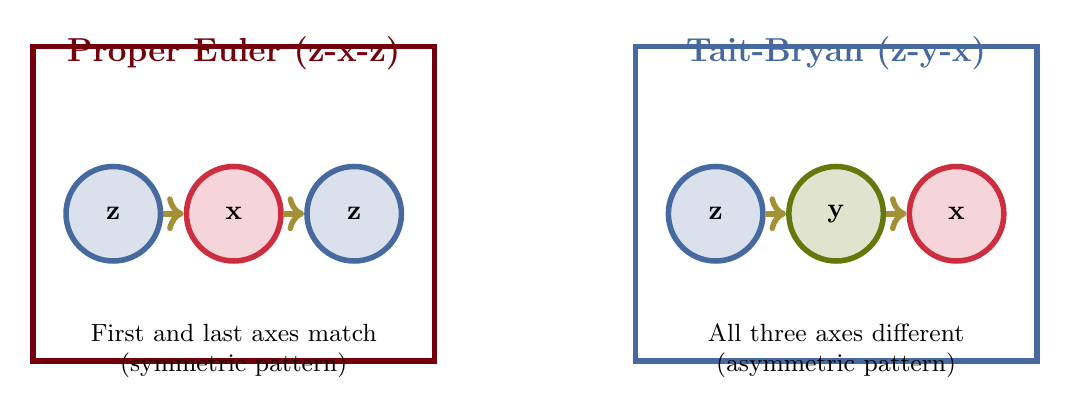
\begin{tikzpicture}[scale=0.85]
    % Proper Euler box
    \begin{scope}[shift={(-4.5,0)}]
        \draw[draw=Garnet, line width=2pt, fill=white] (-3,-2.2) rectangle (3,2.5);
        \node[above, font=\bfseries\large, Garnet] at (0,2) {Proper Euler (z-x-z)};

        % Three circles showing axis sequence
        \node[circle, draw=USC_Blue, line width=2pt, fill=USC_Blue!20, minimum size=1.2cm] (z1) at (-1.8,0) {\textbf{z}};
        \node[circle, draw=USC_Rose, line width=2pt, fill=USC_Rose!20, minimum size=1.2cm] (x) at (0,0) {\textbf{x}};
        \node[circle, draw=USC_Blue, line width=2pt, fill=USC_Blue!20, minimum size=1.2cm] (z2) at (1.8,0) {\textbf{z}};

        \draw[->, line width=2pt, USC_Gold] (z1) -- (x);
        \draw[->, line width=2pt, USC_Gold] (x) -- (z2);

        \node[below, font=\small, text width=5cm, align=center] at (0,-1.5) {First and last axes match\\(symmetric pattern)};
    \end{scope}

    % Tait-Bryan box
    \begin{scope}[shift={(4.5,0)}]
        \draw[draw=USC_Blue, line width=2pt, fill=white] (-3,-2.2) rectangle (3,2.5);
        \node[above, font=\bfseries\large, USC_Blue] at (0,2) {Tait-Bryan (z-y-x)};

        % Three circles showing axis sequence
        \node[circle, draw=USC_Blue, line width=2pt, fill=USC_Blue!20, minimum size=1.2cm] (z) at (-1.8,0) {\textbf{z}};
        \node[circle, draw=USC_Olive, line width=2pt, fill=USC_Olive!20, minimum size=1.2cm] (y) at (0,0) {\textbf{y}};
        \node[circle, draw=USC_Rose, line width=2pt, fill=USC_Rose!20, minimum size=1.2cm] (x2) at (1.8,0) {\textbf{x}};

        \draw[->, line width=2pt, USC_Gold] (z) -- (y);
        \draw[->, line width=2pt, USC_Gold] (y) -- (x2);

        \node[below, font=\small, text width=5cm, align=center] at (0,-1.5) {All three axes different\\(asymmetric pattern)};
    \end{scope}
\end{tikzpicture}
\end{document}
